\section*{Introduction}

This experiment involves the use of a microwave tansmitter and receiver pair to measure the shape of an interference pattern caused by light passing through a double slit.

Unfortunately, this experiment did not proceed as planned due to issues in implementation, but it has given us experimenters a chance to learn about a few of the mistakes we made in its design and execution. This is the price we paid for having successful and accurate experimnents and data throughout the term.

\subsection*{Aim}

We wished to measure the wavelength of a microwave source using a derivative of Young's double-slit experiment.
We also had the intention of using this wavelength and a measured or known frequency to measure the speed of light.

The double slit experiment involves coherent light passing through two rectangular slits in a shield. The resulting diffraction around the edges of each slits produces two curved wavefronts that interfere with each other. When measured on a screen, or in this case, recording the intensity of received radiation at an angle, an interference is revealed where constructive interference produces high intensity spots, and destructive interference produces zero intensity spots. The double slit experiment can be carried out with any radiation, and in fact, anything with wave-like properties, including matter such as electrons, which follows from De Broglie's matter wave theory. It is important that the scale of the experiment is similar to that of the wavelength being tested. In this case, to allow for macroscopic analysis and construction of the experiment, microwaves were used. This allows the experiment to be carried out on an easily perceived scale due to the microwave used having a wavelength in the centimetres.

\subsection*{Relevant Theory}
\label {sec:theory}

Using the wave model of light, we can calculate the expected intensity of light at an angle. The intensity is affected two interferences. The diffraction caused by a single slit, and the interference between both slits' wavefronts. As a note, it is vital that the source light is completely in phase with itself (coherent). This means that every emitted photon shares the same wave equation in both time and space (before diffraction). Uncoherent light will still interfere, but in a completely random way that results in a similarly uniform output with no peaks or valleys, resulting in no observed effect.

Interference is a result of the superposition property. At each point in space, the intensity of the total light wave is the sum of all light waves through that point. Since the propagation of a wave is due to its electric and magnetic waves, we can model the electric wave instead of the light wave. The electric wave is sinusoidal in intensity at a point over time, or at a time over a distance. From the first property, the intensity on a point on the screen will be a sum of these sine waves, itself a sine wave. Therefore it is the points where the source waves are in phase where constructive interference is seen, and where they are out of phase that destructive interference is seen.

By modelling the double slit experiment as two spherically propagating sources of initially in-phase light, any point has a light wave that is the sum of the two sources. The phase difference at any point is therefore given by the relationship between the wavelength, and the path difference at the given point. This results in the equation of intensity 

\begin{equation}
	\label{eqn:DoubleSlitIntensity}
I = I_{max} ~ \cos^2 \left(\frac{\pi \, d \, \sin(\theta)}{\lambda}\right)
\end{equation}

where $d$ is the distance between the two slits, and $\lambda$ is the wavelength.

The derivation of the single slit intensity constructs infinite light sources across a slit of width $a$. The phase difference between the two edges of slit is given by

\begin{equation}
	\label{eqn:SingleSlitPhase}
	\phi = \frac{2 \pi}{\lambda} \, a \, \sin(\theta).
\end{equation}


This results in an equation of intensity

\begin{equation}
	\label{eqn:SingleSlitIntensity}
	I = I_{max} ~ \left( \frac{\sin({\alpha})}{\alpha} \right)^2 \text{ where } \alpha = \frac{\phi}{2}.
\end{equation}

The total intensity at an angle is the product of the reductions in \eqref{eqn:DoubleSlitIntensity} and \eqref{eqn:SingleSlitIntensity}, i.e. 

\begin{equation}
	\label{eqn:Intensity}
I = I_{max} ~ \cos^2{\left(\frac{\pi \, d \, \sin(\theta)}{\lambda}\right)} \left( \frac{\sin({\alpha})}{\alpha} \right)^2.
\end{equation}

The expected curve between angle and intensity is shown below for $\frac{d}{a} \approx 4$.
\begin{figure}[h]
\centering
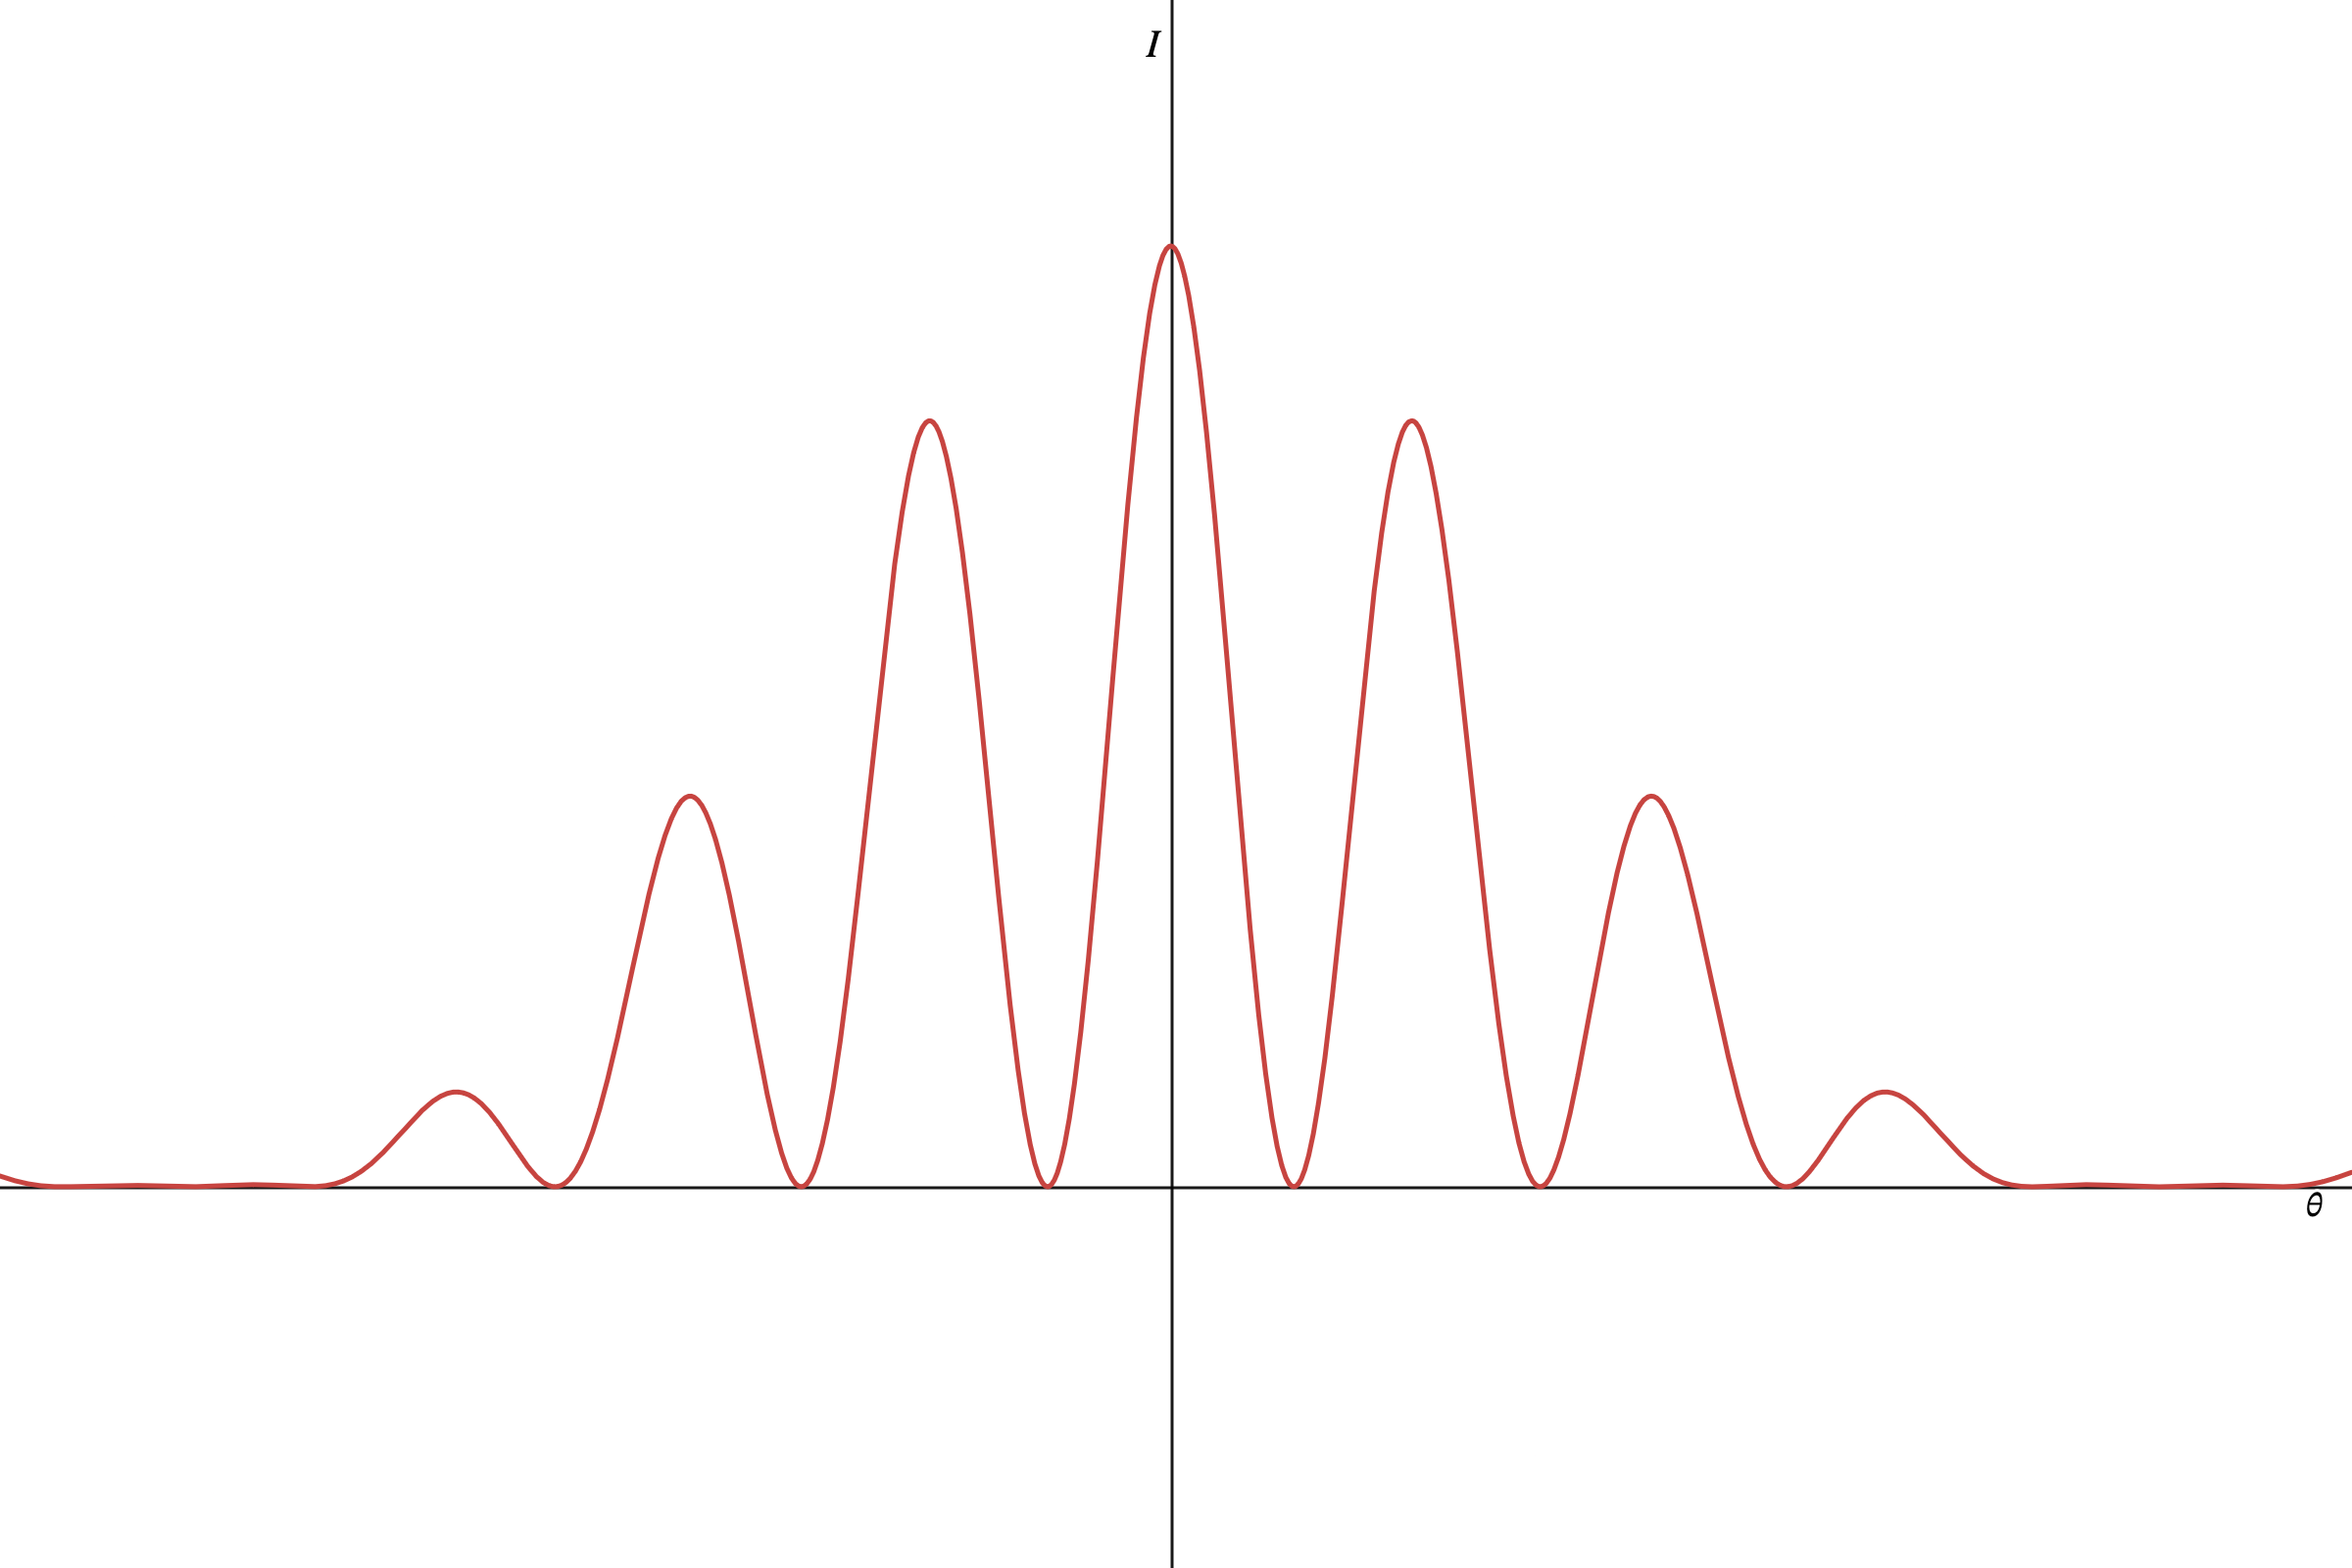
\includegraphics[width=0.4\textwidth]{theory_graph.png}
\caption{Expected curve}
\label{fig:ExpectedCurve}
\end{figure}

\section*{Apparatus}

The experiment used:
\begin{itemize}
\item PASCO microwave transmitter
\item PASCO microwave receiver
\item Goniometer
\item Magnetic strip plate sleds
\item Vernier voltage probe
\item Smart phone (angle sensor)
\item Laptop
\item Logger Pro hardware \& software
\end{itemize}

\subsection*{Setup}

Mount the transmitter and receiver sleds to the goniometer as shown in figure \ref{fig:goniometer_and_microwaves}. The receiver should be on the arm that is free to rotate relative to the central stand.

In the experiment we tried the pair in both their horizontal and vertical orientations, and found that vertical worked better.

The smartphone is used as an angle sensor via its internal accelerometer and magnemometer that it uses for functions such as compass heading. From here it will be referred to as the angle sensor. The angle sensor must be mounted flat, and be rotationally rigid with respect to the microwave receiver. In our experiment, the phone sat in the receiver's sled base, and was kept anchored using a wedge.

Two series of data must be synchronised for this experiment \textemdash time-voltage and time-angle. The time-angle measurement is already designed to store UTC time, but the logger pro software stores time as a duration from the start of the recording. To therefore get the universal time of the voltage, the universal time of at least one voltage data point must be recorded. This was done by constantly displaying the current time at the same time as the voltage data was logged, and screen recording both. Time was displayed using a simple bash script that infinitely printed the current seconds since the UNIX epoch, which was also recorded in the angle data. The below script prints the time every ~5ms which is similar to the polling rate of the angle measurements.


\begin{minted}{bash}
#!/bin/bash
while true
do
    perl -MTime::HiRes -e 'printf("%.3f\n",Time::HiRes::time())'
done
\end{minted}

\begin{figure}[h]
\centering
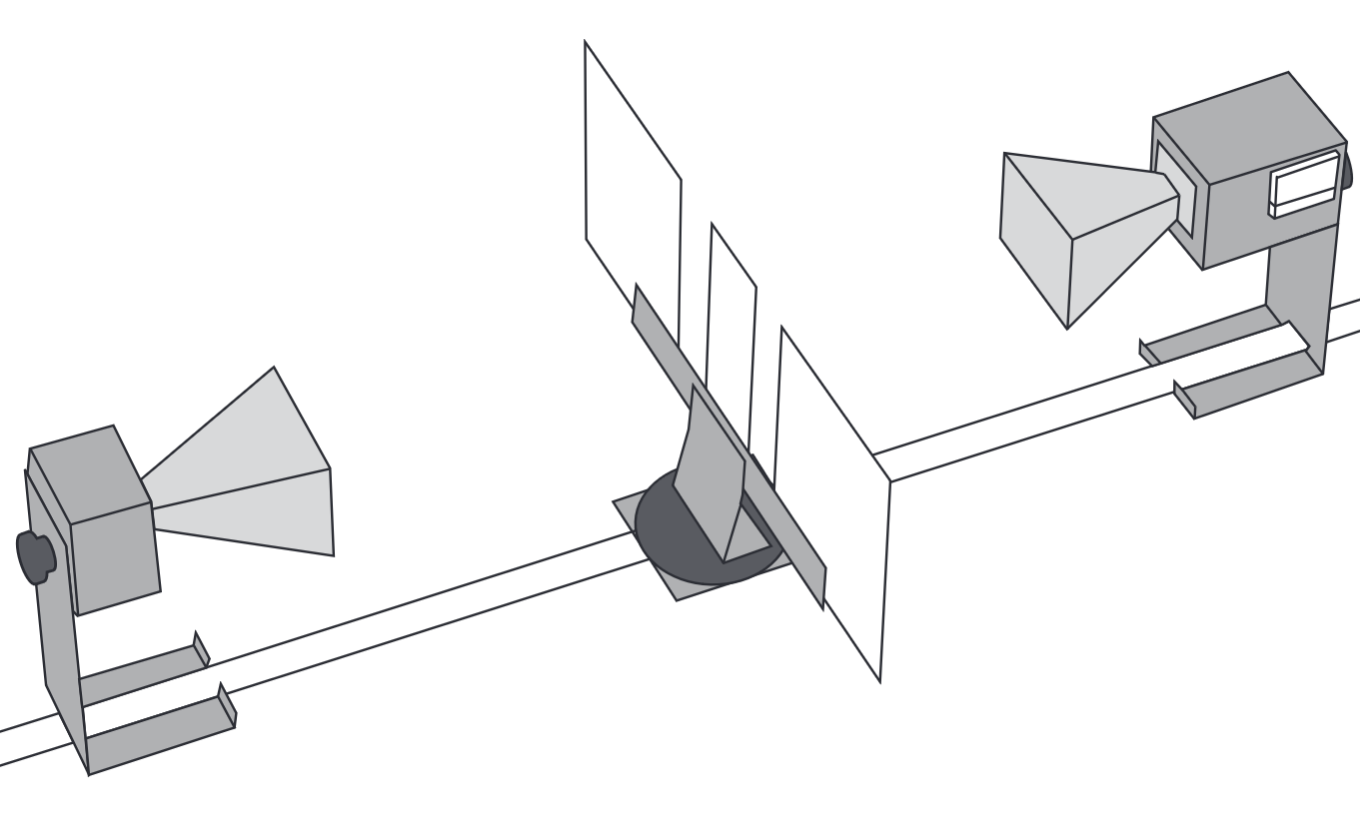
\includegraphics[width=0.5\textwidth]{setup_for_double_slit.png}
\caption{Setup of microwave transmitter/receiver and double slit (credit to PASCO manual)}

\label{fig:goniometer_and_microwaves}
\end{figure}

\subsubsection*{Logger Pro settings}
Set polling rate to 500Hz (1 measurement every 2ms). Set record duration to 120s.

\subsubsection*{Angle Measurement}

The angle of the goniometer was measured in a novel way in this experiment. Since the voltage probe records a constant sample of voltages, something similar was wanted for angle. To solve this, a smart phone's magnetic heading reading was used.

The setup involves a webserver receiving and writing recorded angle measurements, and a web browser taking and sending them. The webserver must be started, while the phone and laptop are on the same local area network. The university network is not completely open and is quite complicated, so the phone's hotspot was use and the laptop was connected to that. This does not use mobile data however, the phone merely acts as a modem. The server can then be restarted and passed a file name to write to. The phone does not have to reload the page, it will keep sending requests even when the server is down between trials. c-
Although this setup seemed to work reliably, it in fact did not work at all, and did not produce usable measurements. The data recorded did not seem to fit at all with the movements that were made. There were stretches of no recorded change in angle, and also stretches where massive fast changes were recorded, both without any relation to the real movement at the time, or the intensity recordings. This was quite strange, because when carrying out the experiment, the live angle indicator always moved in an expected way. In testing of the apparatqus after the experiment, such as through slow and fast 360° rotations, the angle was recorded as expected.

The issues of this apparatus and its integration into the experiment are analysed later in the report.

\section*{Method}

\begin{enumerate}
\item Set up experiment as defined above. Be wary of large flat surfaces that can reflect microwaves, and therefore interfere with the experiment. The microwave transmitter should be placed far enough away from the slits that its light passes through both slits, but not too far that it disperses too much. We found a distance of 30cm worked well.
\item Take out the phone and spin it around in a figure eight so that it resets its orientation and is properly calibrated.
		This step shouldn't be necessary, and would be removed upon improvement of this piece of apparatus as described later.
\item Begin the server writing to a file (\verb|python3 server.py t1.csv|) where t1.csv refers to the current trial.
\item Start the recording on the logger pro software.
\item Slowly sweep the receiving goniometer across its full range of motion.
\item Once the logging has completed, stop the server (ctrl-C) to stop recording angle data.
\end{enumerate}

\section*{Uncertainty Analysis}

There is uncertainty in both series of data:

\subsection*{Angle data}

\subsubsection*{Time measurements}

The time measurements are taken from the phone's OS at the time of measurement. Since humans have spent a lot of time figuring out how to tell the time with computers (computers have nanosecond accuracy to themselves, and microsecond accuracy to each other), the uncertainty in the time measurements will be taken as negligible. There may be a constant systematic uncertainty resulting in all measurements being off by the same amount, but this will be much smaller than the synchronisation error between the two computers.

\subsubsection*{Angle measurements}

It was not possible to find a theoretical accuracy for the relative accuracy of the phone's bearing measurements. Since we only care about change in angle within the dataset, and not the true angle compared to magnetic North, these values are irrelevant. Leaving the phone steady in a stationary environment produced consistent readings up to 2 decimal places, with the 3rd decimal place fluctuating randomly within a 0.005° range. Using this, we have estimated the systematic uncertainty to be 0.01°. 
On average, $\Delta \theta \approx 10\deg$ between two minima, giving $\frac{0.01°}{10°}= 0.1\%$ uncertainty. This seems too low, and it was not practical to rigorously test the device's accuracy, so an error of 3\% will be used.

\subsection*{Voltage measurements}

Time will be the same as above.

The voltage probe has a provided resolution of 1.6mV, although in the data the recorded voltages seemed have ~3mV resolution which is near the probe's 12-bit resolution.
Based on the data however, for any small change in time, i.e. on the order of 10ms, which would include 5 readings, there is a much greater range in voltage than would be expected. This is likely due to noise introduced by the microwave receiver, leading to 
 Although this error is present, the values of the voltage are unimportant in this experiment, only their relative magnitudes.

\begin{wrapfigure}{r}{0.3\textwidth}
	\centering
	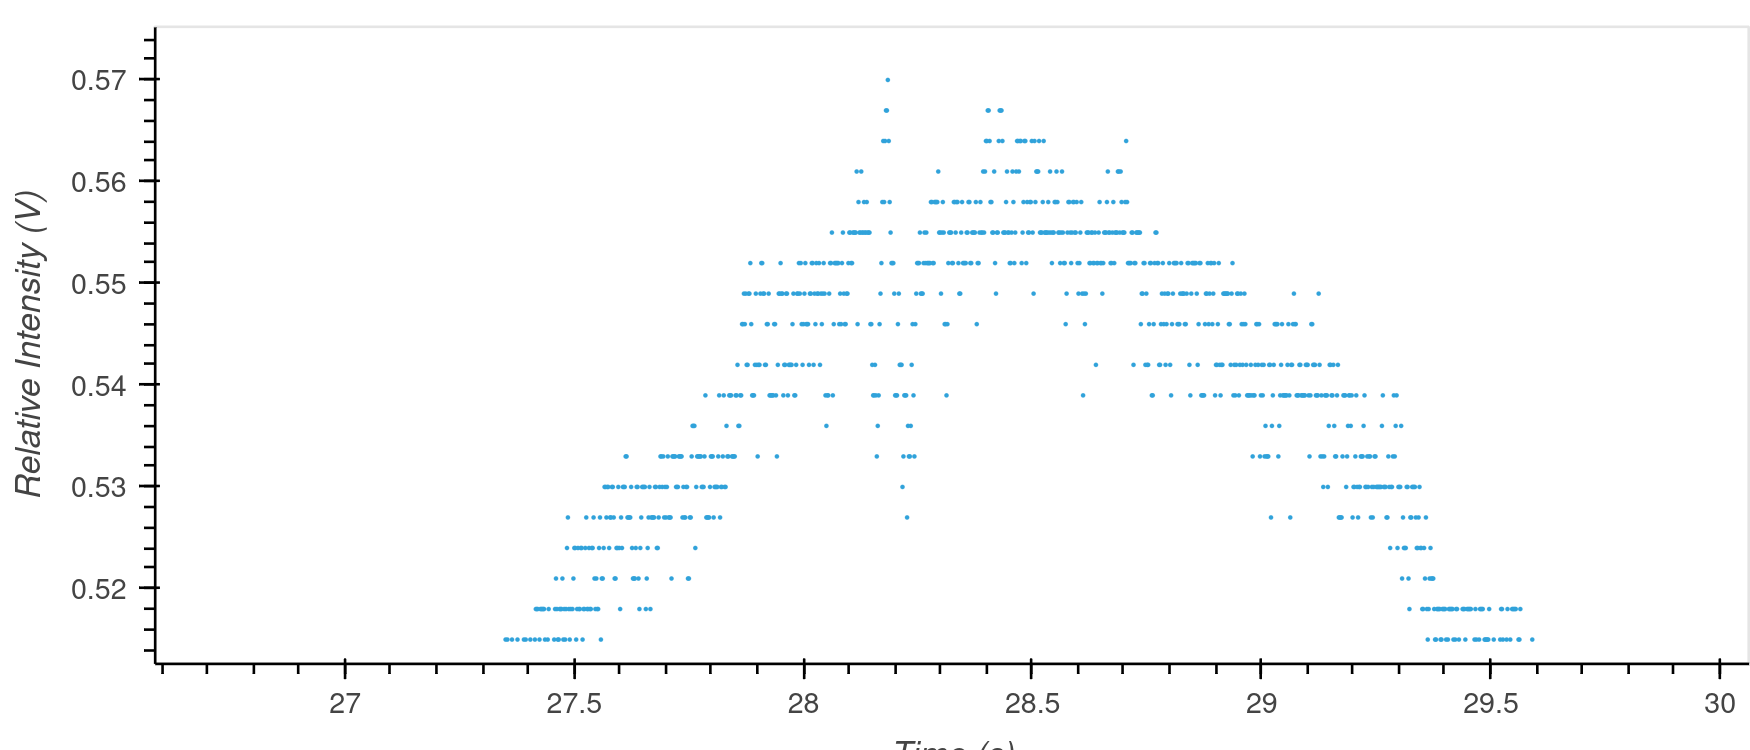
\includegraphics[width=0.3\textwidth]{voltage_line_error_height.png}
	\caption{High zoom into voltage peak data}
\end{wrapfigure} 

The voltage probe has a provided resolution of 1.6mV, although in the data the recorded voltages seemed have ~3mV resolution which is near the probe's 12-bit resolution.
Based on the data however, for any small change in time, i.e. on the order of 10ms, which would include 5 readings, there is a much greater range in voltage than would be expected. This is likely due to noise introduced by the microwave receiver, leading to an error range of the height of the voltage line, which is ~20mV.
 Although this error is present, the values of the voltage are unimportant in this experiment, only their relative magnitudes which allow for the detection of maxima and minima.

\subsection*{Synchronisation}

The two series must be synchronised so that each time-voltage pair can be associated with a time-angle pair, producing an angle-voltage pair. Due to the limited way in which the universal time of the logger pro series could be recorded, we estimate an uncertainty of 5ms in the time. The greatest uncertainty likely comes from the frame rate was 60fps, so ~17ms per frame. This gives an uncertainty of 8ms in the time synchronisation.

The time series were combined using an AsOf left join on the voltage data, which selects the closest matching row. This adds an uncertainty that is related to the resolution of the angle data. The angle data has a time resolution of 5ms, but the procurement of an uncertainty from this process is not obvious, so an estimation of 5\% uncertainty will be made.

Combining these, we have $\sigma_{sys} = \sqrt{ \frac{\Delta t}{t}^2 + \frac{\Delta \theta}{\theta}^2 + \frac{\Delta V}{V}^2 } = 6\%$

\section*{Analysis}

The entire point of taking digitally sampled data for the angle measurement was so that the final angle vs intensity curve could be reconstructed. This would then allow us to fit it to the experimental curve described in \nameref{sec:theory} based on our values of $d$ and $a$. If this did not produce usable results, the contigency was to only inspect the peaks of the graph and their respective angles. This method would be similar to watching the analogue read out for a stationary point, but would allow better accuracy by being able to more accurately determine the real maxima of the curve. This would then allow the deduction of lambda from the equations described before, and also from the interference maxima equation, $d \, \sin(\theta) = m \lambda$.

The analysis itself was done in python using the polars data library. The synchronisation of the voltage series was manually determined using the screen recordings, saved into a table. 
This offset was then added to all the relative time displacements in the voltage series. The time-angle and time-voltage series were then combined using a join 
\verb|combined = intensity.join_asof(angle, on="real_time")| producing the angle-voltage series. These series were then plotted for each trial.

The analysis would have continued to all for a comparison between theoretical and emperical data, however this was not conducted due to the poor data gathered.

The final intention was to determine the wavelength of the microwave, then multiply that with the provided frequency of $10.525 GHz$

\section*{Data}

\subsubsection*{Trial Notes}
\begin{center}
\begin{tabularx}{\linewidth}{ |c | X| }
 \hline
 Trial & Notes \\ 
\hline
 1 & Voltage data not saved \\ 
 2 & Sweep was fast resulting in spiked maxima, making it difficult to determine accurate angle of maximum. \\ 
 3 & Slit distance was increased to test wider slits. \\ 
 4 &  \\ 
 5 & Changed from horizontal horn and polarisation to vertical. This had a positive effect on the results: the resultant graph did not have the same lower bound envelope that was observed in previous trials. Where zeros were expected on higher order minima, the minimum voltage was around 20\% to 50\% of the central maximum. \\ 
 6 &  \\ 
 7 &  \\ 
 \hline
\end{tabularx}
\end{center}

The raw data recorded consists of the time-angle series measured using the angle sensor apparatus, the time-voltage series measured using the Vernier differential voltage probe, and recorded using Logger Pro software, and the screen recording synchronisation data. Both time series consist of a time column and their respective data column, and were polling on the order of 2-5Hz.

The data is represented here post-processed and in plot form. This is because the raw data consists of a large (24MB) of digital sample values, so it would not be reasonable to present here. The data is accessible in the provided git repository in its raw and processed form however.

The synchronisation data that was derived from the screen recordings is in the \nameref{tab:SynchronisationTable}.

The plots are vital to understanding the data due to the sheer quantity of data points recorded; with only numerical aggregations it would be impossilbe to gain an understanding of the experiment.

\begin{figure}

\newlength{\plotwidth}
\setlength{\plotwidth}{0.33\textwidth}


\begin{subfigure}{1.0\textwidth}
\caption*{Trial 2}
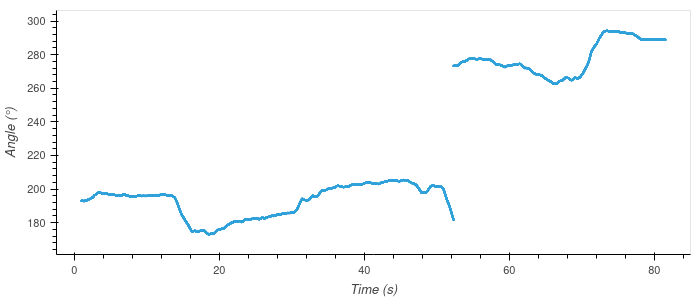
\includegraphics[width=\plotwidth]{plots/t2-time-angle.png}
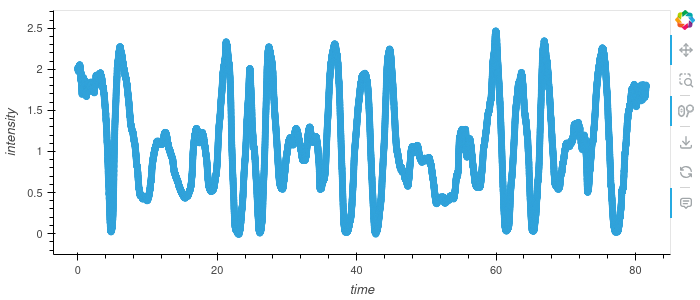
\includegraphics[width=\plotwidth]{plots/t2-time-intensity.png}
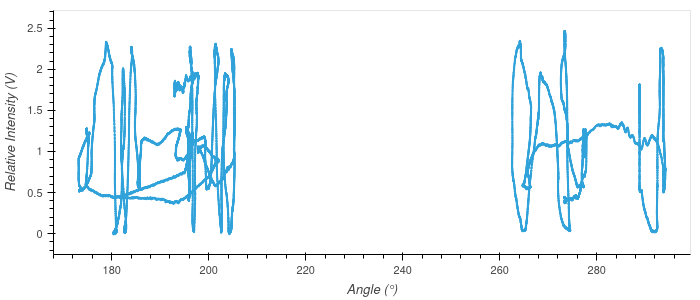
\includegraphics[width=\plotwidth]{plots/t2-angle-intensity.png}
\end{subfigure}



\begin{subfigure}{1.0\textwidth}
\caption*{Trial 3}
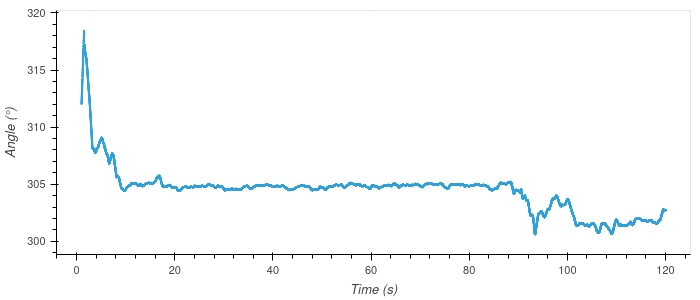
\includegraphics[width=\plotwidth]{plots/t3-time-angle.png}
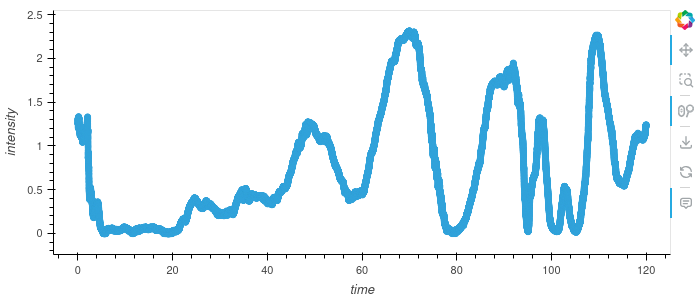
\includegraphics[width=\plotwidth]{plots/t3-time-intensity.png}
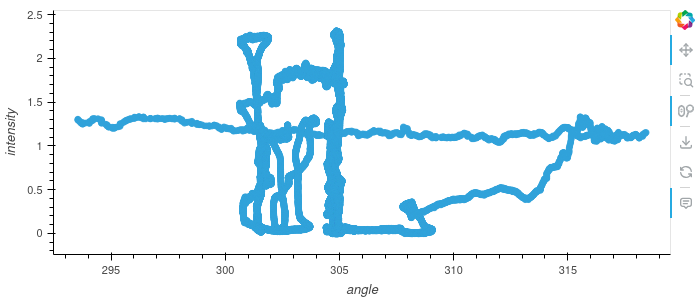
\includegraphics[width=\plotwidth]{plots/t3-angle-intensity.png}
\end{subfigure}



\begin{subfigure}{1.0\textwidth}
\caption*{Trial 4}
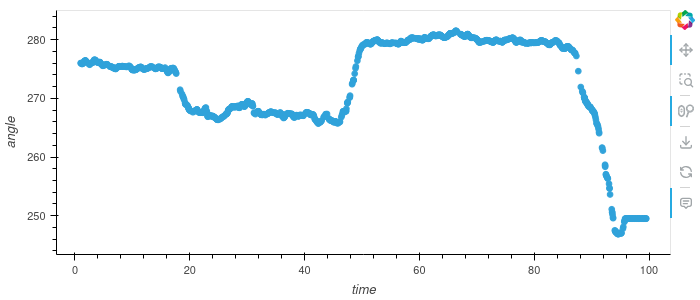
\includegraphics[width=\plotwidth]{plots/t4-time-angle.png}
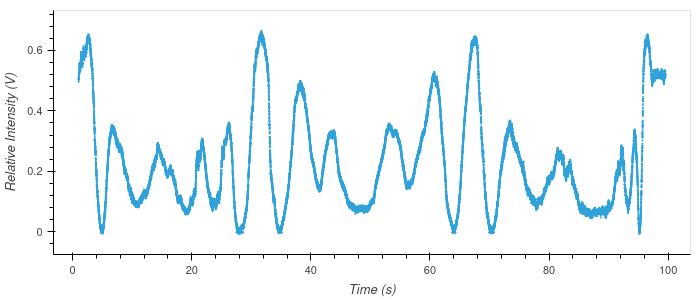
\includegraphics[width=\plotwidth]{plots/t4-time-intensity.png}
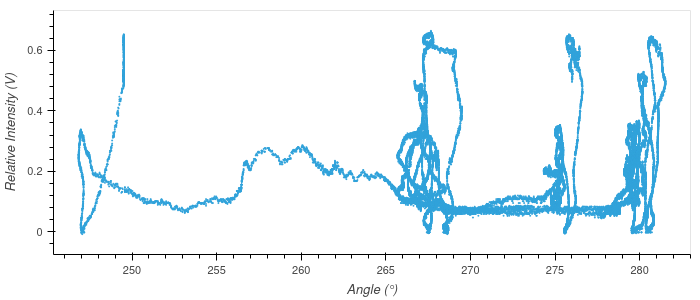
\includegraphics[width=\plotwidth]{plots/t4-angle-intensity.png}
\end{subfigure}



\begin{subfigure}{1.0\textwidth}
\caption*{Trial 5}
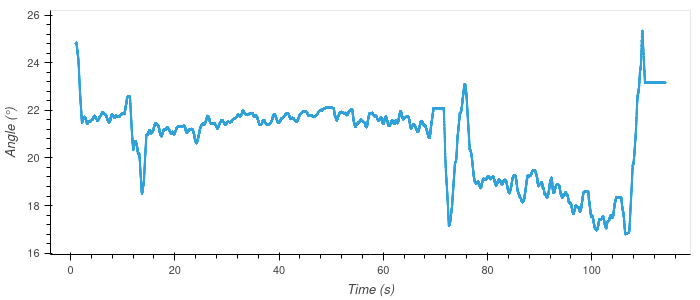
\includegraphics[width=\plotwidth]{plots/t6-time-angle.png}
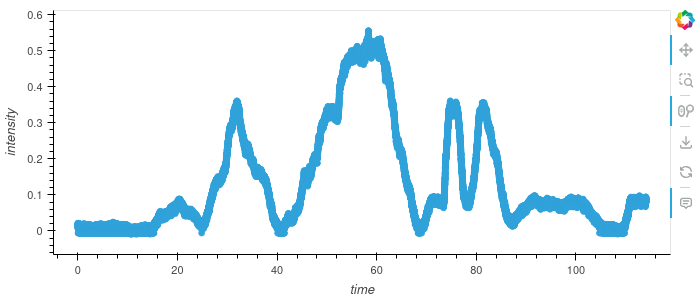
\includegraphics[width=\plotwidth]{plots/t6-time-intensity.png}
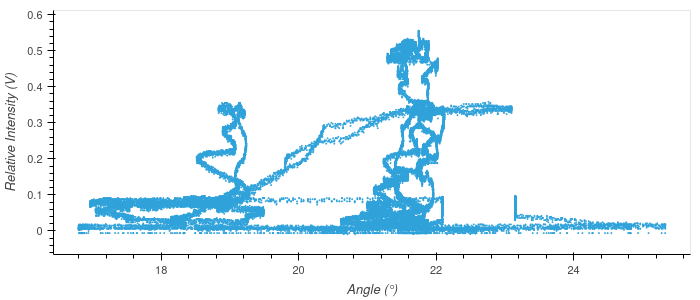
\includegraphics[width=\plotwidth]{plots/t6-angle-intensity.png}
\end{subfigure}



\begin{subfigure}{1.0\textwidth}
\caption*{Trial 6}
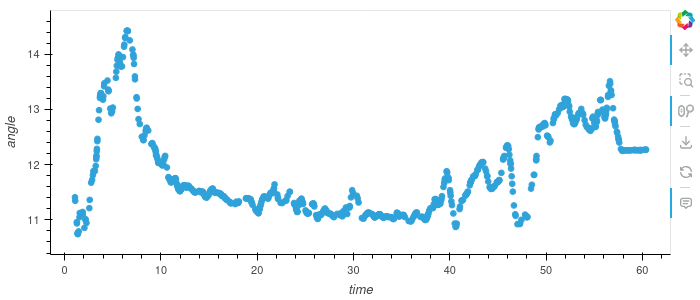
\includegraphics[width=\plotwidth]{plots/t7-time-angle.png}
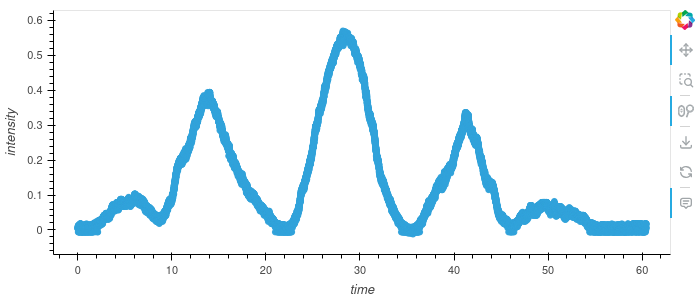
\includegraphics[width=\plotwidth]{plots/t7-time-intensity.png}
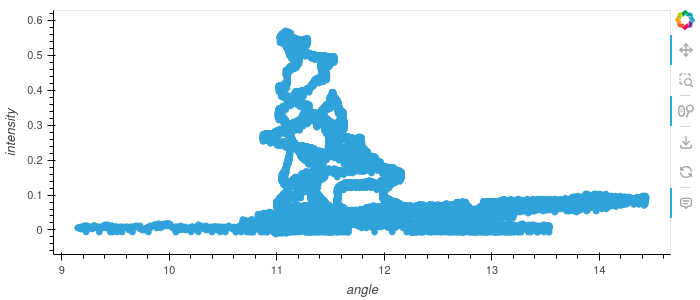
\includegraphics[width=\plotwidth]{plots/t7-angle-intensity.png}
\end{subfigure}



\begin{subfigure}{1.0\textwidth}
\caption*{Trial 7}
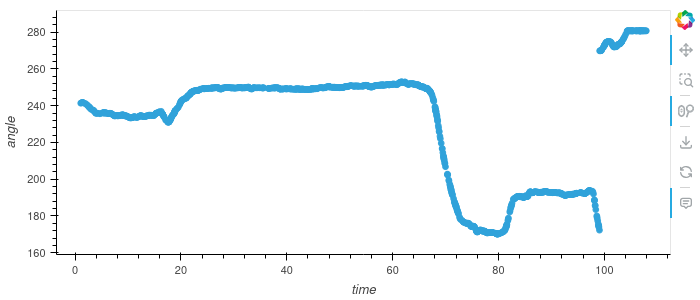
\includegraphics[width=\plotwidth]{plots/t8-time-angle.png}
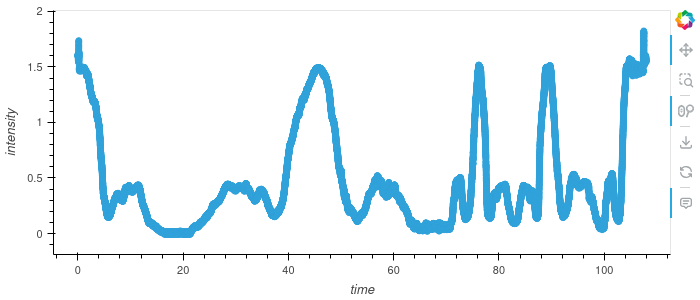
\includegraphics[width=\plotwidth]{plots/t8-time-intensity.png}
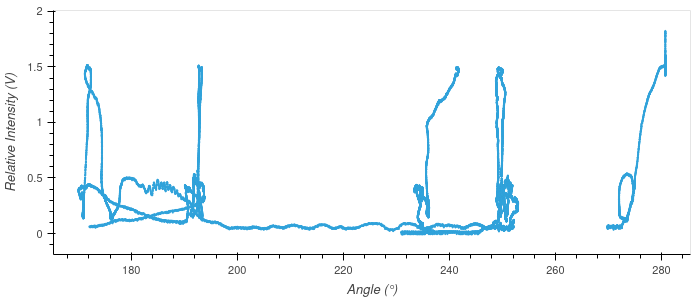
\includegraphics[width=\plotwidth]{plots/t8-angle-intensity.png}
\end{subfigure}

\caption{
Left to right: time versus angle, time versus intensity, combined seres — angle versus intensity\\
Top to bottom: Trials 2 through 7
}
\end{figure}


\section*{Results}

As hinted throughout the report, this section was not as kind to write. 

As is obvious in the last column of the results, the experiment failed to produce usable data. The following post-mortem will explore some of the reasons we think this occurred.

\subsection*{Analysis}

This is the source of bad data. By comparing the plots of angle over time to the movement carried out during the experiment, we see that the recorded angle has seemingly no bearing on reality. This was quite a confusing and frustrating discovery since during testing and upon cursory inspection during the experiment the angle measurement seemed to operate correctly. 
In some of the trials such as 3, 4, 5, there are plateaus of angle where there is still change in voltage. This should not occur and is indicative of the sensor's catastrophic failure. There are also periods of fast and spiked changes in angle, (trials 3, 4, 5) which does not correlate with the slow rotation carried out during the experiment.

It is also important to note that the starting angle and overall range varies greatly. This is unexpected as although Earth hasn't had one for a long time, geomagnetic reversal is quite slow. This aspect of the data leads into our questioning of the sensor's calibration and reliability.

The discontinuities are expected as the sensor measures in a range of $[0°, \, 360°)$.

The failure of the measurement is most obvious in the angle-voltage data. Comparing these plots with the expected curve (figure \ref{fig:ExpectedCurve}) will result in a migraine, and we were thus unable to draw any valid conclusion from the data about the phenomena we attempted to measure. Referencing the previously calculated uncertainty, I can confidently say that our result was not consistent.

\subsection*{Discussion}



\section*{Appendix}


\begin{table}
\subsubsection*{Synchronisation Offsets}
Below is the table of synchronisation used to combine the angle and voltage time series. This is also \verb|time_sync.csv| in the repository.
For each trial, there is a universal time that was determined manually using the screen recording described in the setup instructions.
\label{tab:SynchronisationTable}
\begin{center}
\begin{tabular}{|lrr|}

\hline
Trial & Time displacement of sync (s) & Universal time of sync (milliseconds since the Unix Epoch) \\
\hline
2 & 0.008 & 1722394505249 \\
3 & 0.008 & 1722394831805 \\
4 & 0.016 & 1722395699363 \\
6 & 0.008 & 1722396690634 \\
7 & 0.008 & 1722396880177 \\
8 & 0.008 & 1722397031178 \\
\hline
\end{tabular}

\end{center}
\end{table}

\subsection*{Code}

The raw data, code, and latex source are available on a public GitHub repository.
The analysis scripts require \verb|python3|, \verb|Flask|, \verb|hvplot|, and \verb|polars| for the webserver, plotting, and analysis.
The rendered graphs are also available, including the vector based plots that allow high precision zooming and interaction.

Repo: \href{https://github*.com/TunaMaestro/phys1241_final_lab.git}{\text{https://github.com/TunaMaestro/phys1241\_final\_lab.git}}




